\documentclass[12pt, twoside]{report}
\usepackage[utf8]{inputenc}
\usepackage[margin=2.5cm]{geometry}
\usepackage{graphicx}  		% display images
\usepackage{rotating}
\usepackage{tikz} 
\usepackage[portuguese]{babel}

\usepackage{mathptmx}
\usepackage{setspace}

\usepackage[colorlinks=true,linkcolor=black,urlcolor=blue,bookmarksopen=true]{hyperref} % Make hyperlinks in index
\usepackage{bookmark} 		% Bookmarks for pdf file
\usepackage{float} 			% colocar as imegens e tabelas dentro do texto
\usepackage{fancyhdr}
\pagestyle{fancy}
\usepackage{tabularx} 		% x column in table can jump a line
\usepackage{setspace} 		% espçamento entre linhas
\usepackage{fancyhdr} 		% creates fancy footers and headers
\raggedbottom				% makes bottom of page more empy to make sure previous text doesnt have vertical gaps
\usepackage{ltablex}
\usepackage{pdflscape}
\usepackage{multirow}
\usepackage{minted} %colocação de códigos
\pagestyle{fancy}
\lfoot{{\footnotesize Tecnologias de Informação}}
\rfoot{{\footnotesize ESTGA}}
\rhead{PTDW}
\lfoot{Calendário de exames}
\usepackage{nomencl}
\makenomenclature
\renewcommand{\nomname}{Nomenclatura}%mudar o nome da secção

\renewcommand{\footrulewidth}{1pt}%criar uma linha no que separa o rodapé

\renewcommand\listoflistingscaption{Índices dos comandos e configurações} %lista dos codigos



\begin{document}
	
\onehalfspacing % espaçamento de 1,5 entre linhas

	\pagenumbering{roman}
	
	\begin{titlepage}
		\centering
		\scshape\Huge Calendário Exames\par
		\vspace{0.9cm}
		
		\scshape\large Projeto em Tecnologias da Informação \\
		\vspace{0.3cm}
		\scshape\large 1º semestre de 2021/2022\par
		\vspace{0.4cm}
		\centering
		
		\vspace{3cm}
		
		\large
		Autor\\
		Sofia Rocha, Nº 99991 \\
		
		\vspace{2cm}
		\large
		Águeda, mês, 2022 \\
		
		\vspace{4cm}
		
		\centering
		
\includegraphics[width=10cm]{image/AssB_vertical_cor.png}
		
		
		\newpage
		\thispagestyle{plain}%retira cabeçalho e rodape
		\thispagestyle{empty}%retira a numeração da pagina
		\centering
		\scshape\Huge Calendário Exames \par
		\vspace{1cm}
		
		\scshape\large Projeto em Tecnologias da Informação\par
		\vspace{1cm}
		\scshape\large 2º semestre de 2021/2022\par
		\vspace{4cm}
		
		\large
		Autor\\
		Sofia Rocha, Nº 99991 \\
		
		\vspace{1cm}
		Orientador\\
		Fábio Marques\\
		
		\vspace{3cm}
		\large
		Águeda, mês, 2022 \\
		
		\vspace{2cm}
		\centering
		
\includegraphics[width=10cm]{image/AssB_vertical_cor}
		
	\end{titlepage}

	\begin{abstract}
	\setstretch{1.5}
	\setlength{\parskip}{14pt}
	\setlength{\parindent}{0pt}
	
	
	Resumo máximo 300 palavras
	palavras-chave (6 no máximo)
	\end{abstract}
	
	\begin{abstract}
		Resumo em inglês máximo 300 palavras
		palavras-chave (6 no máximo)
	\end{abstract}

	\newpage
	\setcounter{page}{1} % começa a contar a paginas no numero 1
	\tableofcontents % Índice de conteúdos
	\thispagestyle{plain} % retira cabeçalho e rodape
	\thispagestyle{empty} % retira a numeração da pagina
	\newpage
	\listoftables % Lista de tabelas
	\newpage
	\listoffigures % Lista de figuras
	
	
	\newpage
	\pagenumbering{arabic}
	

	\chapter{Introdução}
	\setstretch{1.5}
	\setlength{\parskip}{14pt}
	\setlength{\parindent}{0pt}
Apresentação do tema do estágio/projeto e da EA;
Apresentação dos objetivos gerais e específicos do estágio/projeto;
Indicação da metodologia de trabalho adotada
Descrição da estrutura interna do relatório

	
	\chapter{Planificação do projeto}
	Identificação e descrição das atividades previstas para a realização
	do projeto (Plano de Trabalho)
	\section{Revisão do estado do projeto}
	
		Antes de começar a implementar novas funcionalidades foi feita uma revisão de todo o projeto, a partir dos requisitos identificados no semestre passado (ver tabela \ref{requisitiosfuncionaisrevisao}), para identificar que funcionalidades necessitavam de revisões e correções de erros e quais não foram implementadas do planeamento inicial.
		
		
	\def\arraystretch{1.5}
	\begin{center}
		\label{requisitiosfuncionaisrevisao}
		\begin{longtable}{|m{1cm}|m{2.2cm}|m{9cm}|m{3cm}|}
			\caption{Requisitos funcionais implementados e não implementados}\\
			
			\hline			
			\textbf{Refª }	& \textbf{Categoria}&\textbf{Descrição do requisito} & \textbf{Implementado?} \\
			\hline
			
			RF.1 &Importação& Importação de ficheiros com a configuração de salas, disciplinas e docentes em formato \textbf{csv} & Sim \\
			\hline
			
			RF.2 &\multirow{2}{2cm}{Exportação}& Exportação de calendários em formato \textbf{pdf} & Não \\
			
			RF.3 && Exportação o calendário em língua inglesa & Não \\
			\hline
			
			RF.4 &\multirow{3}{2cm}{Marcação de exames}& Os exames podem ser marcados em três turnos: às 9h30, às 14h e às 18h30 & Sim \\
			
			RF.5 && Associação de um ou mais vigilantes a cada exame & Não \\
			
			RF.6 && O calendário não deverá permitir a marcação de exames aos domingos e feriados & Não \\
			
			RF.7 &&	Associação de uma ou mais salas a cada exame & Não\\
			
			RF.8 && Se houver vários cursos com o mesmo exame então será associado a todos os calendários dos cursos associados. & Não\\
			\hline
			
			RF.9 &\multirow{7}{2cm}{Configurações}& Configuração do tipo de sala (informática, laboratório de redes e normal) e lotação máxima & Não \\
			
			RF.10 & & Inserção de cursos e disciplinas & Não\\
			
			RF.11 && Permitir inserir novos docentes & Não\\
			
			RF.12 && Permitir editar informações (nome, que disciplinas está a lecionar, horário de trabalho) sobre os docentes & Não\\
			
			RF.13 && Permitir editar informações (nome do curso, docente e a disciplina) sobre as disciplinas e cursos & Não\\
			
			RF.14 && Alterar a disponibilidade dos docentes & Não\\
			
			RF.15 && Permitir colocar restrições arbitrárias introduzidas pelo utilizador & Não \\
			\hline	
			
			RF.16 &\multirow{9}{2cm}{Avisos}& Aparecimento de um aviso no caso de incongruência da informação durante a marcação de exames & Não \\
			
			RF.17 &&Mostrar um aviso de alta prioridade se houver sobreposições de exames & Não\\
			
			RF.18 && Mostrar um aviso de alta prioridade se o docente não estiver disponível & Não \\
			
			RF.19 && Mostrar um aviso de alta prioridade se a sala não estiver disponível & Não\\
			
			RF.20 && Mostrar um aviso de alta prioridade se o curso for diurno e colocar um exame no turno da noite e vice-versa & Não\\
			
			RF.21&&Mostrar um aviso de alta prioridade se o docente associado ao mesmo exame for repetido & Não \\
			
			RF.22 && Mostrar um aviso de alta prioridade se o exame necessitar de uma sala de informática e não for associada sala desse tipo & Não\\
			
			RF.23 && Mostrar um aviso de alta prioridade se houver mais alunos inscritos do que  lotação máxima da sala & Não\\
			
			RF.24 && Mostrar um aviso de média prioridade se houver exames marcados no mesmo dia e hora do mesmo curso mas anos diferentes & Não\\
			
			
			RF.25 && Mostrar um aviso de média prioridade se o utilizador tentar exportar um calendário sem exames marcados & Não\\
			\hline
			
			RF.26 &Autenticação& O utilizador só pode aceder à aplicação após a autenticação & Sim\\
			\hline
			
			RF.27 &\multirow{3}{2cm}{Criação de calendários}&Criação de calendários associados a um curso, ano letivo, ano do curso, época e semestre.& Sim \\
			
			RF.28 && Criação de épocas de avaliação adicionando um nome e uma data de início e fim & Não \\
			
			RF.29 && A criação de um novo calendário deverá sempre partir do início sem exames marcados & Sim\\
			\hline
			RF.30 &\multirow{2}{*}{Histórico}& Guardar e visualizar calendários de exames de anos anteriores (histórico)& Não \\
			
			RF.31 && Filtrar o histórico por curso, ano letivo, ano do curso, semestre e época& Não \\
			\hline
		\end{longtable}
	\end{center}
	
	Apesar de haver várias funcionalidades implementadas algumas destas necessitavam de correção de \textit{bugs}, apresentado na tabela \ref{revisaodaaplicacaobugs}, que prejudicavam a segurança da aplicação ou o comprometimento da funcionalidade. Os requisitos relacionados são referentes à tabela \ref{requisitiosfuncionaisrevisao}.
	
		\begin{table}[H]
		\caption{Requisitos que têm \textit{bugs}}
		
		\begin{center}
			\begin{tabularx}{\textwidth}{|X|X|}
				\hline
				\textbf{Descrição do \textit{bug}} & \textbf{Req. relacionado} \\
				\hline
				O utilizador consegue aceder à aplicação sem autenticação através do url & RF.26\\
				\hline
				Aparece várias vezes o mesmo ano do curso & RF.27\\
				\hline
				Não importa se tiver mais de um professor & RF.1\\
				\hline
				Não verifica se tem dados na base de dados & RF.1\\
				\hline
			\end{tabularx}
			\label{revisaodaaplicacaobugs}
		\end{center}
	\end{table}
	
	\section{Planeamento do projeto}
	
	A partir da revisão feita anteriormente foi possível planear todo o projeto como se pode verificar na figura 
	\ref{planeamentoinicial}.
	
		\clearpage
	\begin{landscape}
		\pagestyle{empty}
		
		\begin{figure}[H] 
			\centering 			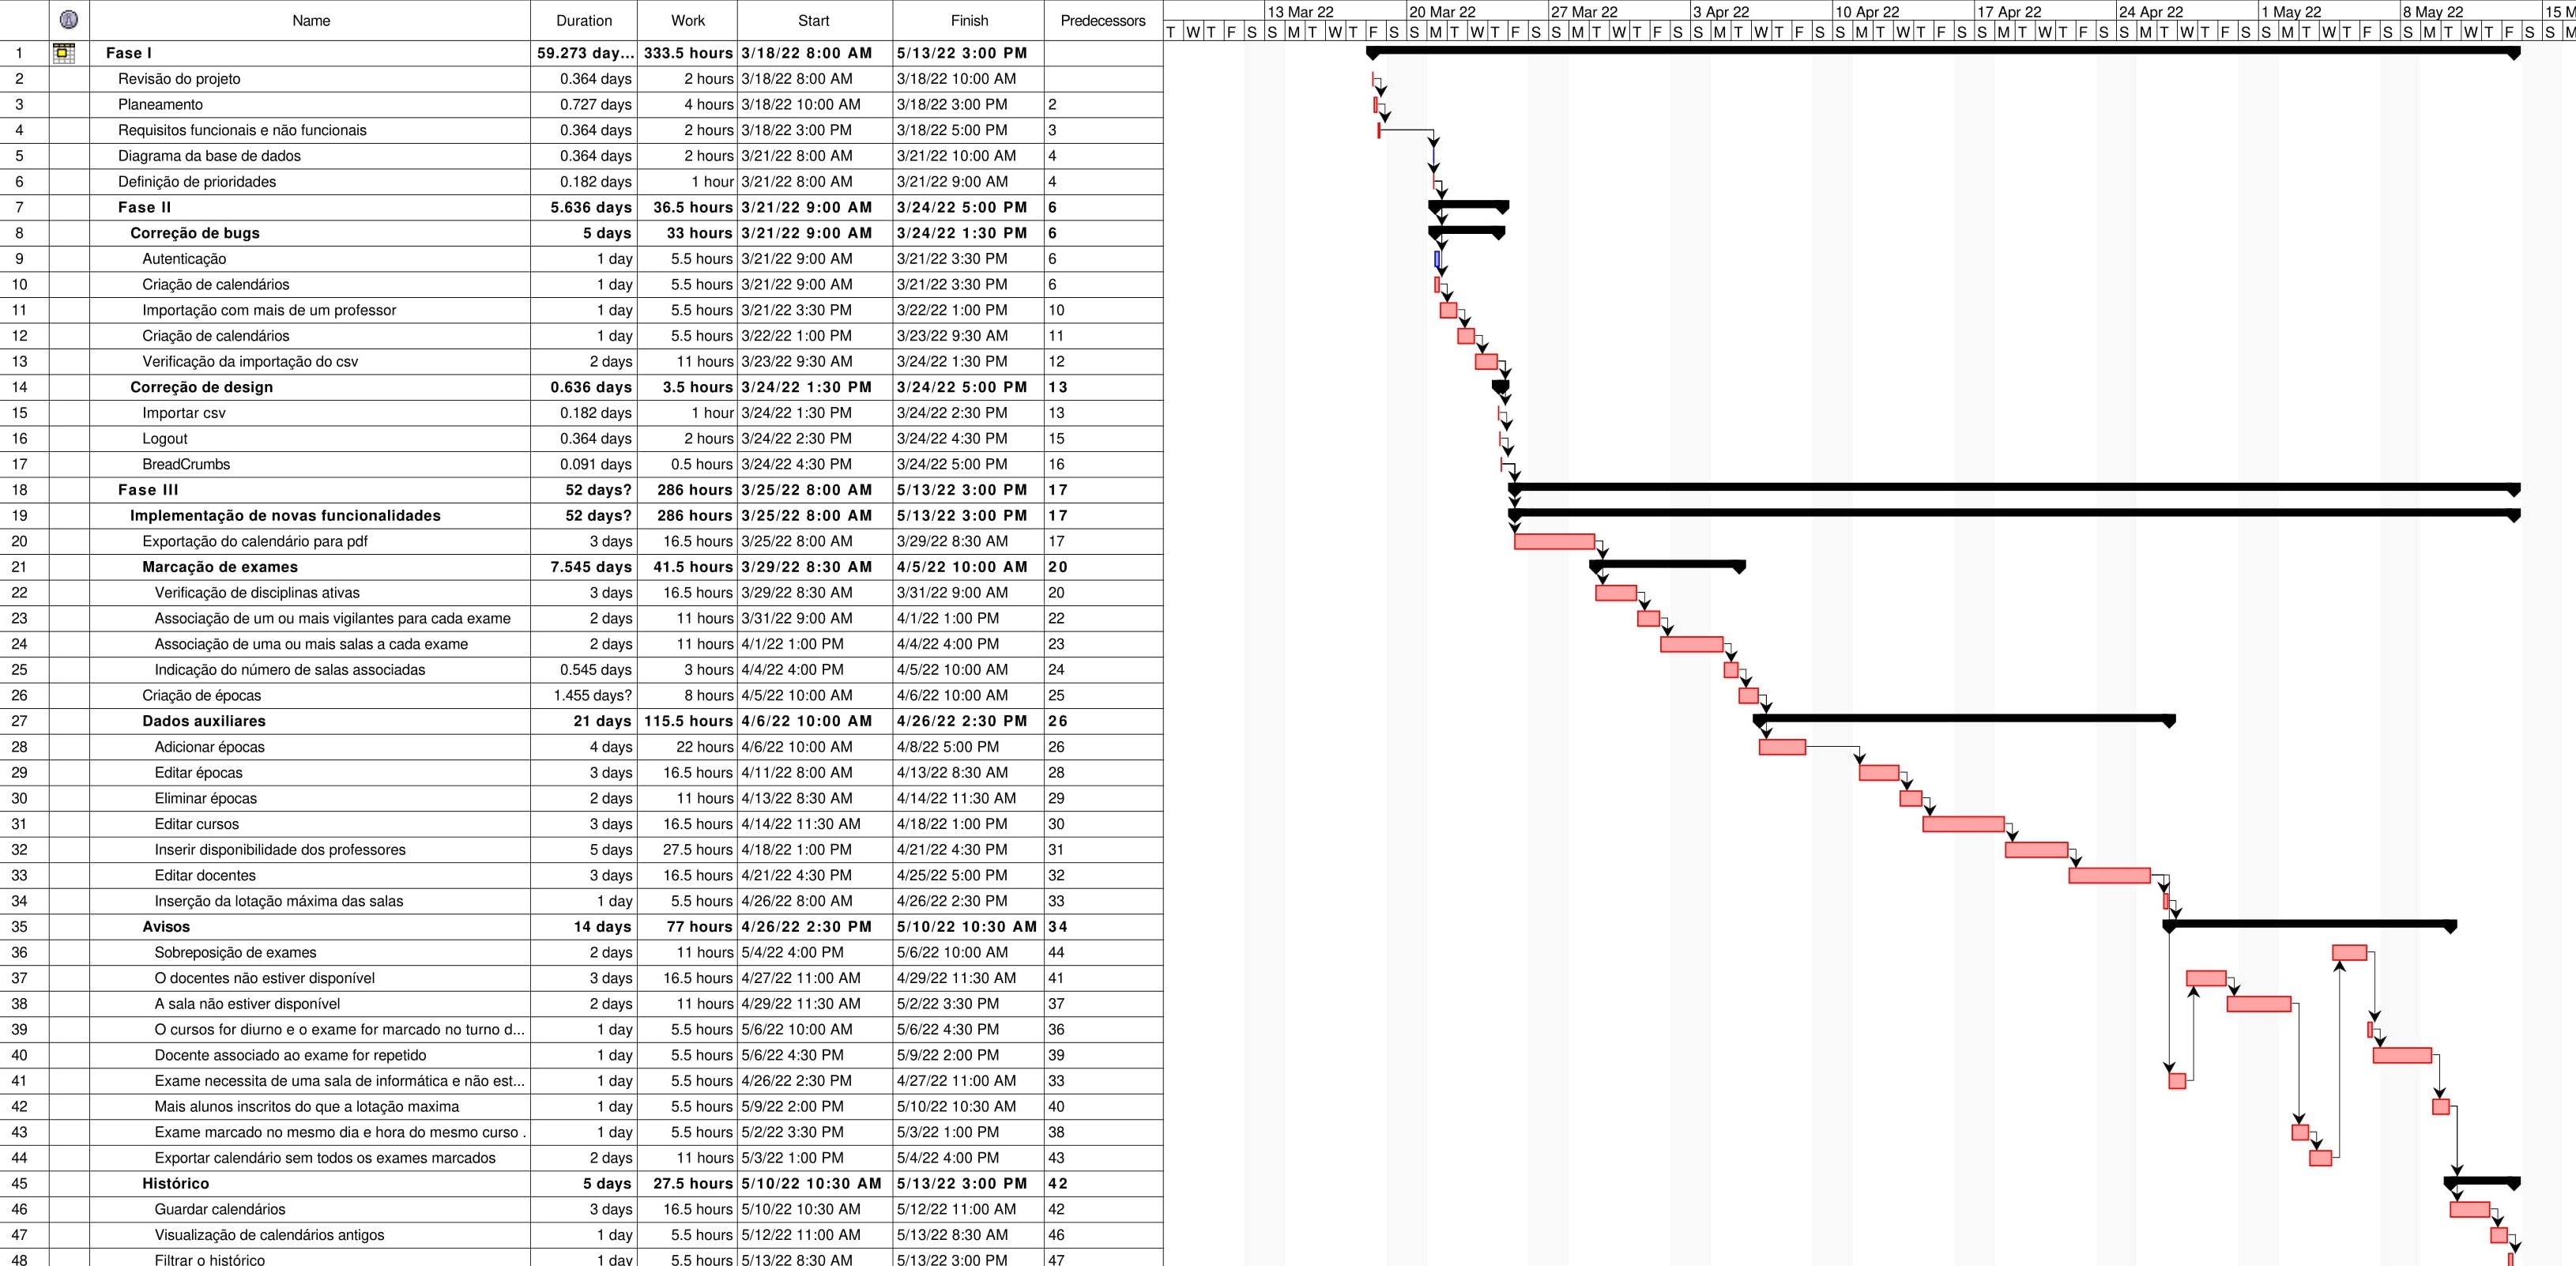
\includegraphics[width=1.4\textwidth,height=1.4\textheight,keepaspectratio]{image/planeamentoInicial}
			\caption{Planeamento do projeto}
			\label{planeamentoinicial}
			
		\end{figure}
		
		
	\end{landscape}
	\chapter{Modelo de requisitos}
	\label{requisitos}
	\section{Requisitos funcionais}
	
	Como este projeto é uma continuação de um projeto anterior então na tabela \ref{requisitiosfuncionais} não se encontram todos os requisitos funcionais, mas sim aqueles que serão implementados. 
	
	
\def\arraystretch{1.5}
	\begin{center}
		\label{requisitiosfuncionais}
		\begin{longtable}{|m{1cm}|m{2.2cm}|m{10cm}|m{2cm}|}
			\caption{Requisitos funcionais a serem implementados}\\
			
			\hline			
			\textbf{Refª }	& \textbf{Categoria}&\textbf{Descrição do requisito} & \textbf{Prioridade} \\
			\hline
			
			
			RF.1 &Importação& Importação de ficheiros com a configuração de salas, disciplinas e docentes em formato \textbf{csv} com dois ou mais docentes& Alta \\
			\hline
			
			RF.2 &\multirow{2}{2cm}{Exportação}& Exportação de calendários em formato \textbf{pdf} & Alta \\
			
			RF.3 && Exportação o calendário em língua inglesa & Baixa \\
			\hline
			
			RF.4 &\multirow{2}{2cm}{Marcação de exames}& Associação de um ou mais vigilantes a cada exame & Alta\\
						
			RF.5 &&	Associação de uma ou mais salas a cada exame & Alta\\
			
			RF.6 &&Indicação do número de salas associadas & Alta\\
			\hline
		
			RF.9 &\multirow{6}{2cm}{Dados Auxiliares}& Inserção da lotação máxima das salas& Média \\
			
			RF.10 && Alterar a disponibilidade dos docentes & Alta\\
			
			RF.10 && Adicionar épocas & Alta\\
			
			RF.11 && Editar épocas & Média\\
			
			RF.12 && Eliminar épocas & Alta\\
			
			RF.13 && Inserir disponibilidade dos docentes & Alta\\
			\hline
			
			RF.16 &\multirow{9}{2cm}{Avisos}& Mostrar um aviso de alta prioridade se houver sobreposições de exames & Baixa\\
						
			RF.17 && Mostrar um aviso de alta prioridade se o docente não estiver disponível & Média \\
			
			RF.18 && Mostrar um aviso de alta prioridade se a sala não estiver disponível & Média\\
			
			RF.19 && Mostrar um aviso de alta prioridade se o curso for diurno e colocar um exame no turno da noite e vice-versa & Baixa\\
			
			RF.20&&Mostrar um aviso de alta prioridade se o docente associado ao mesmo exame for repetido & Alta \\
			
			RF.21 && Mostrar um aviso de alta prioridade se o exame necessitar de uma sala de informática e não for associada sala desse tipo & Alta\\
			
			RF.22 && Mostrar um aviso de alta prioridade se houver mais alunos inscritos do que  lotação máxima da sala & Baixa\\
			
			RF.23 && Mostrar um aviso de média prioridade se houver exames marcados no mesmo dia e hora do mesmo curso mas anos diferentes & Média\\
			
			RF.24 && Mostrar um aviso de média prioridade se o utilizador tentar exportar um calendário sem todos os exames marcados & Média\\
			
			\hline
			
			RF.25 &Autenticação& O utilizador só pode aceder à aplicação após a autenticação & Alta\\
			\hline
			
			RF.26 &\multirow{1}{2cm}{Criação de calendários}& Criação de épocas de avaliação adicionando um nome e uma data de início e fim & Alta \\
	
			\hline
			RF.30 &\multirow{2}{*}{Histórico}& Guardar e visualizar calendários de exames de anos anteriores (histórico)& Média \\
			
			RF.31 && Filtrar o histórico por curso, ano letivo, ano do curso, semestre e época& Média \\
			\hline
		\end{longtable}
	\end{center}



	
	\section{Requisitos não funcionais}
	
	Os requisitos não funcionais estão divididos em três categorias: requisitos de interface e facilidade de uso que representam todos os requisitos que melhorem a usabilidade da aplicação; requisitos de segurança e integridade dos dados e requisitos de interface com sistemas externos e ambientes de execução.
	
	\subsection{Requisitos de interface e facilidade de uso}

Assim que o utilizador inicia a sessão na aplicação este tem de facilmente entender como a aplicação está organizada.
Isto permite que o utilizador utilize a aplicação durante mais tempo e gerir os calendários de avaliações não seja frustrante.
	
	\begin{table}[H]
	\caption{Requisitos de interface e facilidade de uso}
	
	\begin{center}
		\begin{tabularx}{\textwidth}{|c|X|c|}
			\hline
			\textbf{Refª }	& \textbf{Descrição do requisito} & \textbf{Prioridade} \\
			\hline
			RIF1 & As disciplinas e cursos podem ser inseridas através de \textit{drag e drop} &Alta\\
			\hline
			RIF2 & Interface responsivo permitindo a sua visualização em ambiente mobile &Alta\\
			\hline
			RIF3 & Linguagem padrão em Português de Portugal &Alta\\
			\hline
			RIF4 & Há dois tipos de avisos distinguidos com texto e cor &Alta\\
			\hline
		\end{tabularx}
		\label{requisitosdeinterface}
	\end{center}
	\end{table}

	\subsection{Requisitos de segurança e integridade dos dados}
	
	Para que o utilizador possa colocar os seus dados na aplicação sem conter risco de vazar para utilizadores indesejados foram criados alguns requisitos de segurança referido na	tabela \ref{requisitosdeseguranca}.
	
\begin{table}[H]	
	\caption{Requisitos de segurança e integridade dos dados}
	
	
	\begin{center}
		\begin{tabularx}{\textwidth}{|c|X|c|}
			\hline
			\textbf{Refª }	& \textbf{Descrição do requisito} & \textbf{Prioridade} \\
			\hline
			RSI1 &O histórico não pode ter associações a outras tabelas da base de dados  &Alta\\
			\hline
			RSI2 & Uma única conta de utilizador&Alta\\
			\hline
		\end{tabularx}
		\label{requisitosdeseguranca}
	\end{center}
\end{table}


	\subsection{Requisitos de interface com sistemas externos e ambientes de execução}
	
	A aplicação por ambiente da disciplina irá ser programada em linguagens web,
	consequentemente não é necessário definir que sistema operativos pode a aplicação ser executada.
	No entanto é crucial ter acesso à rede da Universidade de Aveiro e um dos navegadores definidos na tabela \ref{requisitosdesistemas}.
	
	\def\arraystretch{1.5}
	\begin{table}[H]
		\caption{Requisitos de interface com sistemas externos e ambientes de execução}
		\begin{center}
			\begin{tabularx}{\textwidth}{|c|X|c|}
				\hline
				\textbf{Refª }	& \textbf{Descrição do requisito} & \textbf{Prioridade}\\
				\hline
				RSA1 & Suportar Browsers com motor renderização webkit/blink (Chrome, Edge, Safari, Brave, etc.)  & Alta \\
				\hline
				RSA2 & Suportar Firefox ESR e outros derivados de gecko/quantum & Alta \\
				\hline
				RSA5 & Estar conectado à rede da Universidade de Aveiro & Alta\\
				\hline
			\end{tabularx}
			\label{requisitosdesistemas}
		\end{center}
	\end{table}
		
	

	
	
	\chapter{Modelo de dados persistentes}
	
		Para cumprir com as novas funcionalidades, apresentados anteriormente na secção \ref{requisitos}, a base de dados teve de ser alterada. 
	
	\section{Estrutura da base de dados}
	
	Para a preparação da aplicação a tabela ``course" é preenchida com todos os cursos da universidade a partir da própria \textit{framework} assim como ``time\_slot" que contém somente os três blocos em que se pode marcar um exame (manhã, tarde e noite).
	
	De seguida, Para utilizar a aplicação o utilizador terá de se autenticar com a sua conta (se não tiver terá de se registar) que está registada na tabela ``users". No entanto não existe nenhuma associação dos dados às contas sendo que todas as contas têm acesso ao mesmos dados.
	
	Depois o utilizador terá de importar o csv em que os dados serão guardados nas tabelas ``professor", ``subject" e ``classroom". Se existir mais que um professor para uma disciplina, estes serão guardados na tabela ``professor", mas só será associado à disciplina o primeiro que aparece no ficheiro .csv uma vez que se assume que é o representante da mesma.
	
	???????????????
	E as salas não são associadas uma vez que na época de exames não existe aulas. (ver o que fazer com os cursos de ctesp) 
	
	Com isto todos os calendários criados serão armazenados na tabela ``calendar" que contém duas chaves estrangeiras para a época e para o curso para os quais foram associados. As épocas (criadas pelo utilizador) são identificadas pelo seu nome, data de início e fim. Para cada calendário existe inúmeros exames que podem ser marcados (tabela ``evaluation\_slot´´) consoante o curso associado. Cada exame tem três chaves estrangeiras: uma para o calendário, outra para a disciplina e outra para o momento do dia em que será a avaliação e um atributo para o dia marcado.
	
	Nesta fase foi alterada a base de dados criando duas tabelas - ``observing\_professor", que guarda todos os vigilantes associados a um exame, e ``associated\_classroom", que armazena todos as salas de um exame - para que possa ser associado um ou mais vigilantes ou uma ou mais salas a cada exame (RF.2 e RF.3 da tabela \ref{requisitiosfuncionais}).
	
	\clearpage
	\begin{landscape}
		\pagestyle{empty}
		
		\begin{figure}[H] 
			\centering 			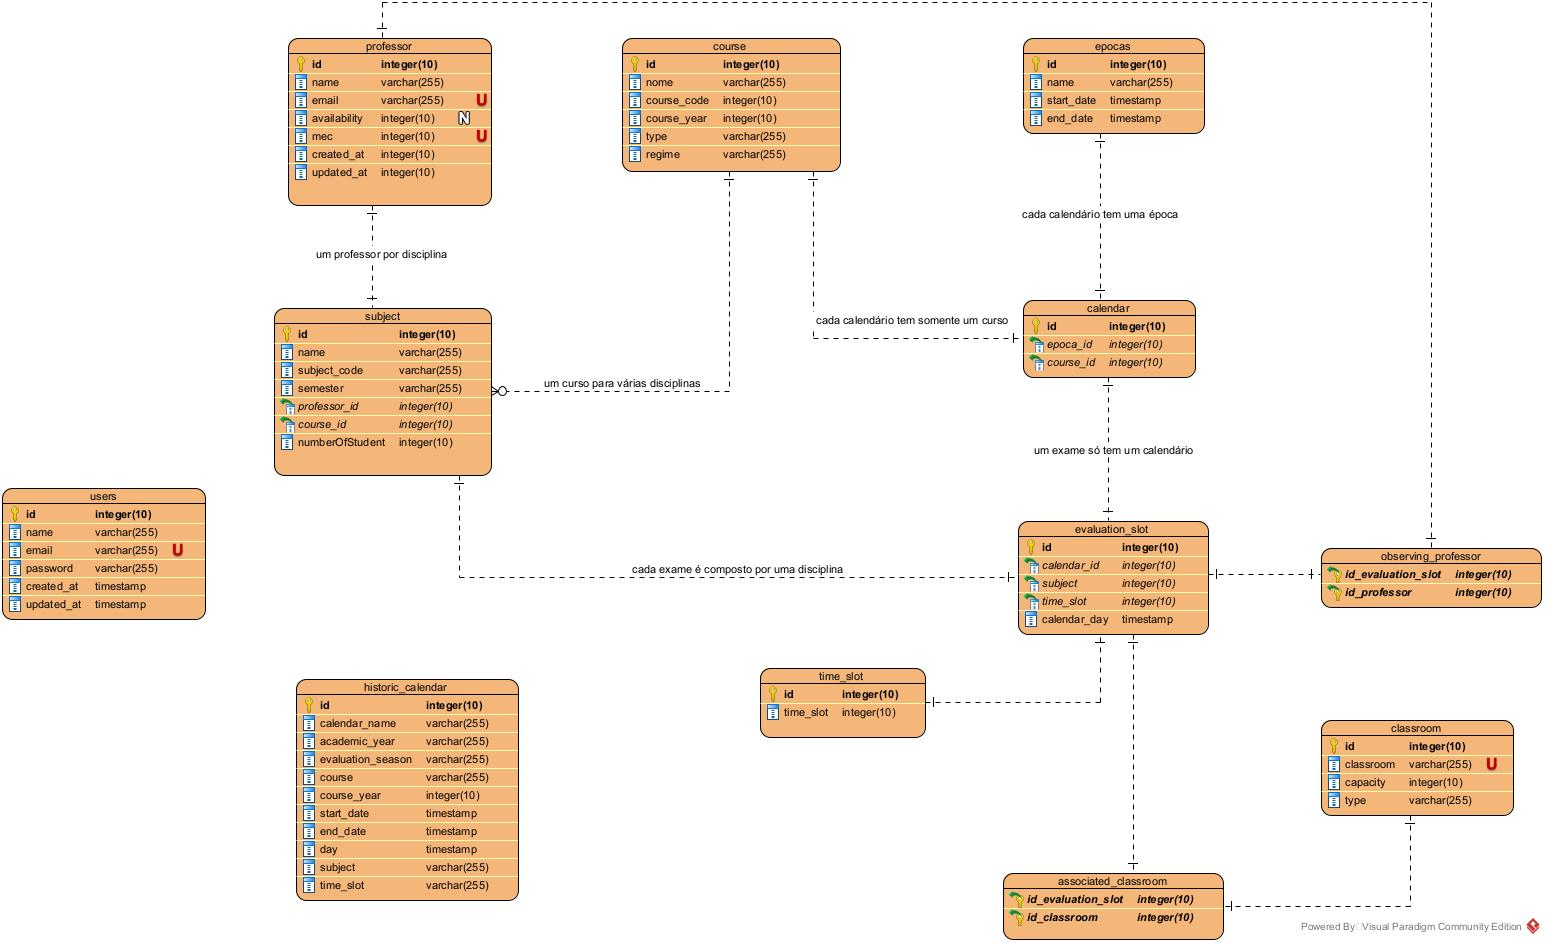
\includegraphics[width=1.4\textwidth,height=1.4\textheight,keepaspectratio]{image/databaseDiagram}
			\caption{Diagrama da base de dados}
			\label{planeamentoinicial}
			
		\end{figure}
		
		
	\end{landscape}
	
	\section{Arquitetura do sistema - modelo MCV}
	
	
	\section{Correção de erros}

	\subsection{Autenticação}
	No começo foi bloqueado o acesso à aplicação através do próprio do url do website. Por exemplo era possível aceder à página de marcação de exames digitando "/marcacao-exames" sem iniciar sessão. 
	Consequentemente, de forma a corrigir este problema, antes de aceder a qualquer rota (exceto a de login e de registo) é verificado se existe uma sessão aberta através do \textit{middleware}, como se pode verificar no código \ref{routesMiddl} e \ref{autenticarMiddl}.
	
	\begin{listing}[H]
	\begin{minted}{php}
	Route::middleware([Authenticate::class])->group(function (){
	
	\end{minted}
	\caption{Verificação através do \textit{middleware} se o utilizador está autenticado}
	\label{routesMiddl}
	\end{listing}                                 
		
	\begin{listing}[H]
	\begin{minted}{php}
	class Authenticate extends Middleware
	{
	/**
	* Caso o utilizador não esteje logado não permite navegar pelas páginas
	* return route
	*/
	protected function redirectTo($request)
	{
	  if (!Auth::check()) {
		return route('login');
	  }
	}
	}
				\end{minted}
				\caption{\textit{Middleware} que redireciona para a página delogin se não tiver autenticado}
				\label{autenticarMiddl}
			\end{listing}    
		
	\subsection{Importação}
	
	Na versão anterior do projeto não se considerava as disciplnas que contivessem mais de um professor, assumindo-se que o ficheiro .csv a importar nunca tivesse esta restrição. No entanto o ficheiro dado contém disciplinas com um professor representante e dois auxiliares. 
	
	Com isso o código foi alterado para verificar se existe mais de um número mecanográfico por disciplina. Se existir o primeiro será assumido como representando da disciplina sendo o único que será associado à mesma e os outros serão somentes guardados na base de dados, como está ilustrado no código \ref{importarprof}. 
	

	\begin{listing}[H]
	\begin{minted}{php}
	$mec = explode(",", $data[$i][9]);
			
	if (count($mec) > 1) {
		$name = explode(",", $data[$i][7]);
		$email = explode(",", $data[$i][8]);
				
		for ($x = 0; $x < count($mec); $x++) {
			//cria um professor ou atualiza o prof 
			se tiver o mesmo número mecanografico
			Professor::updateOrCreate([
			'mec' => $mec[$x],
			'name' => $name[$x],
			'email' => $email[$x],
			]);
		}
	}
	\end{minted}
	\caption{Importação do professores}
	\label{importarprof}
	\end{listing}
	
	\section{Verificação da importação do csv}
	
	Para o utilizador saber se já foi importado um csv este é avisado através de uma mensagem (\textit{toastr}) na página de importar o csv. 
	
	\begin{figure}[H] 
	\centering
	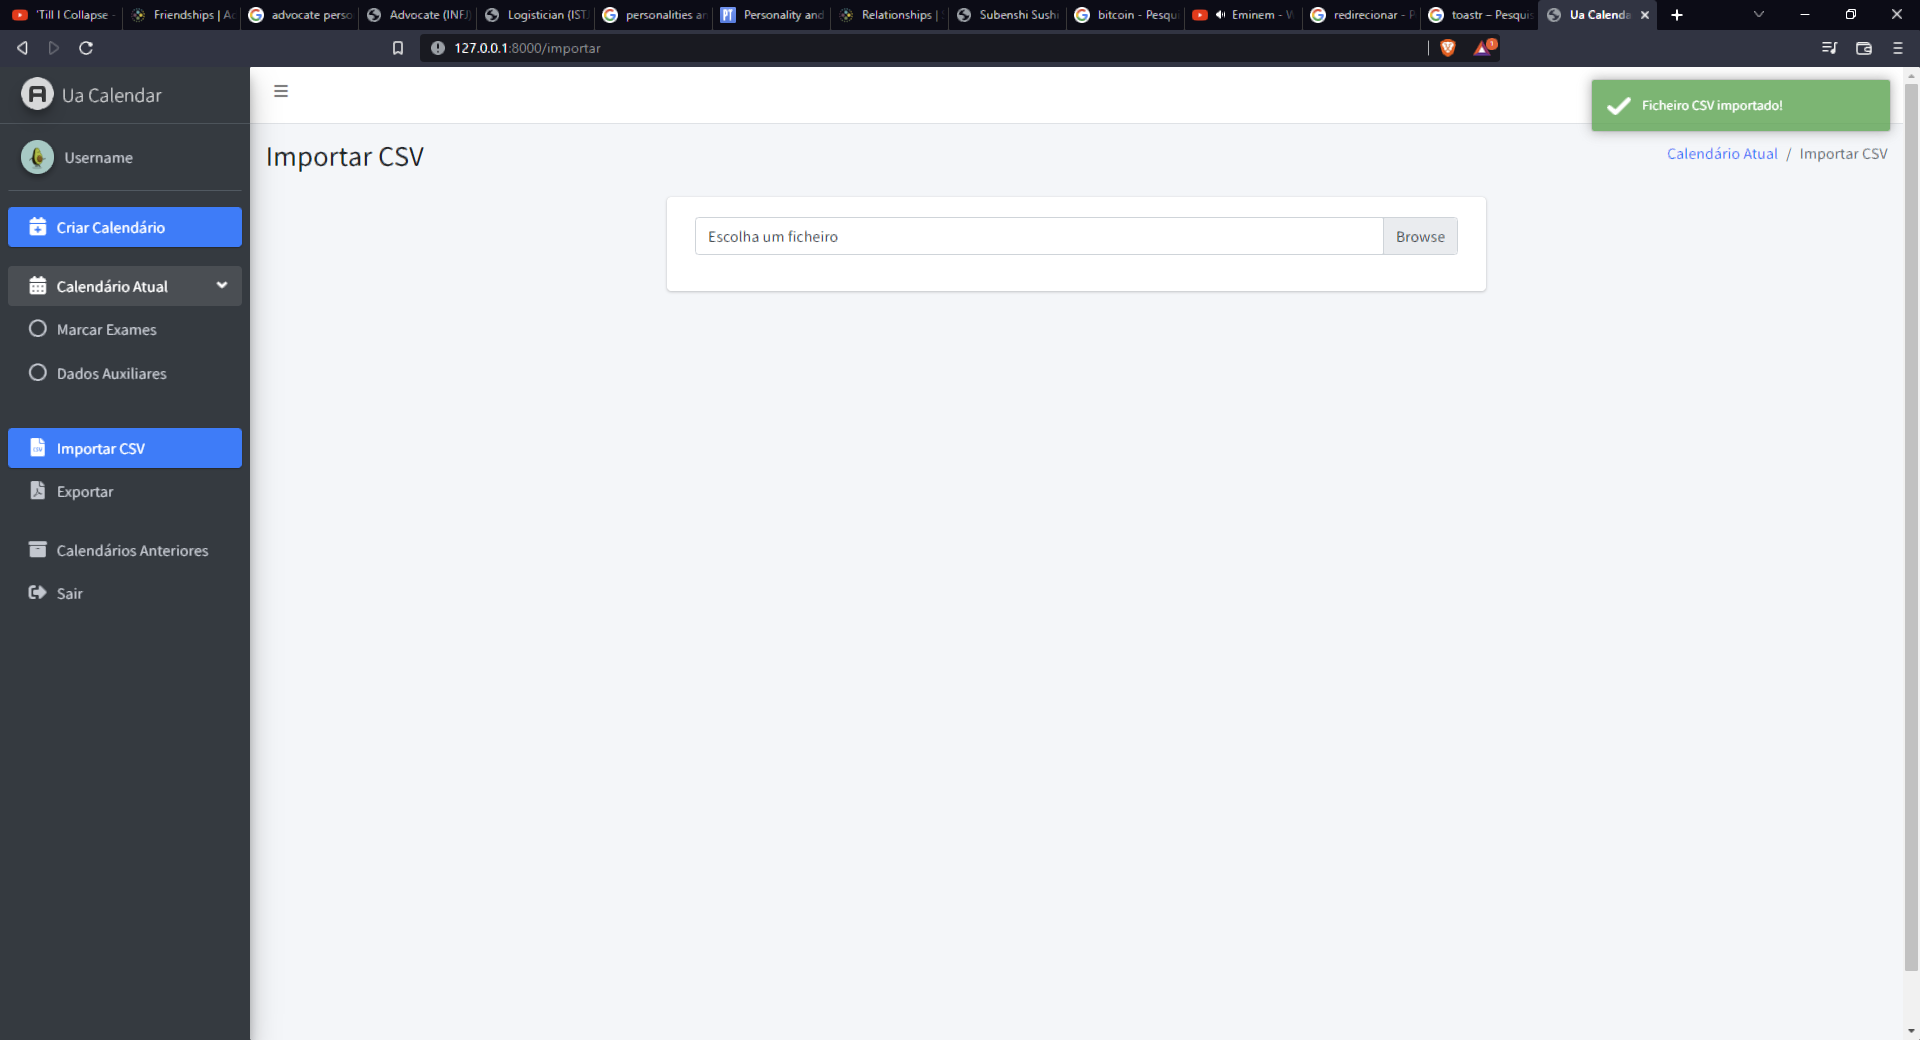
\includegraphics[width=1\textwidth,height=1\textheight,keepaspectratio]{image/importarCSV}
	\caption{\textit{Toastr} de sucesso}
	\label{importarCSVSucess}
		
	\end{figure}

	\begin{figure}[H] 


	\centering 			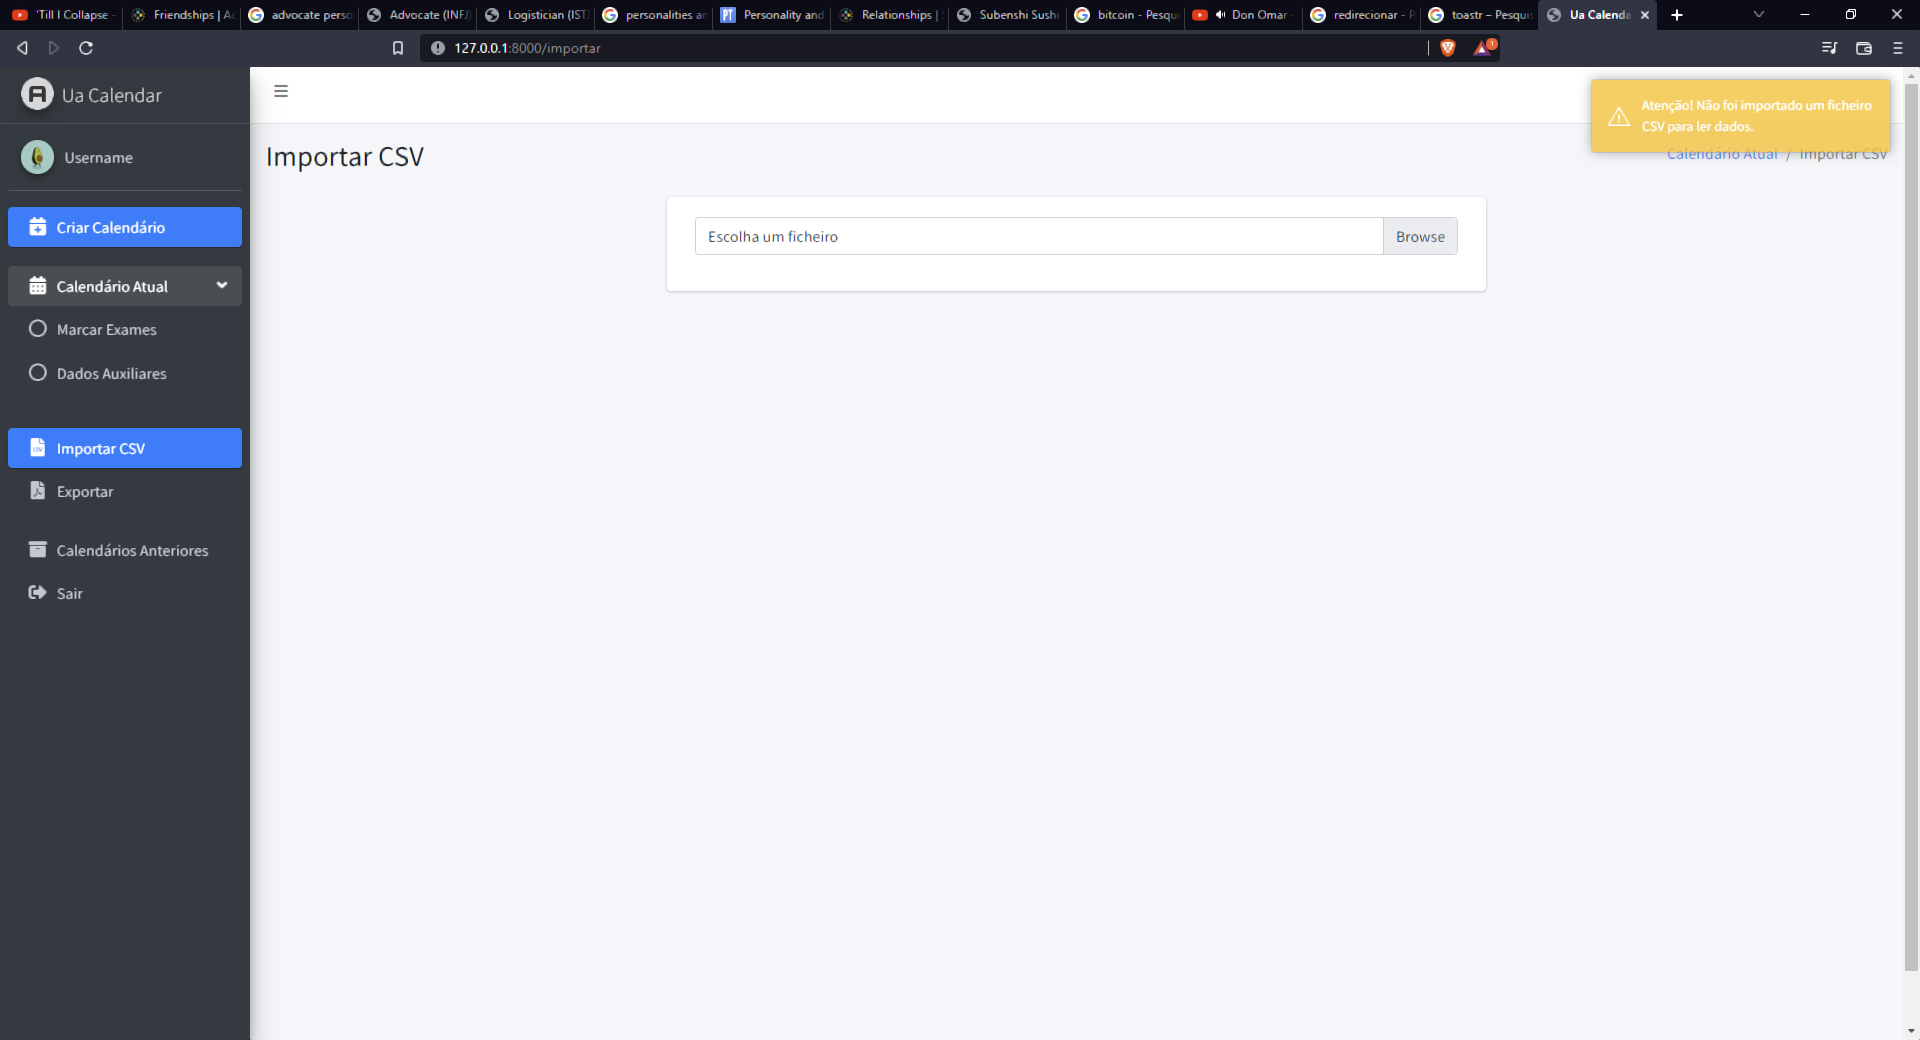
\includegraphics[width=1\textwidth,height=1\textheight,keepaspectratio]{image/importCSVFail}
	\caption{\textit{Toastr} de não ter sido importado um csv}
	\label{importarCSVFail}
	
	\end{figure}

	Este \textit{toastr} é ativado consoante os dados persentes na \textit{cookie} presente. Ao carregar a página é verificado se existe dados na base de dados através do \textit{controller} e com isso é alterado o cookie de acordo com o resultado. Como a tabela de professores é umas das que é preenchida ao importar o ficheiro .csv então se existir dados na mesma quer dizer que este ficheiro ja foi importado, através do código \ref{checkIfImported}. Apesar disto nada impede que importar mais do que uma vez.
	
	\begin{listing}[H]
		\begin{minted}{php}
		/**
		* Verifica se o csv já foi importado
		* @return bool
		*/
		public function checkIfImported()
		{
			if (Professor::exists())
			return true;
			
			return false;
		}
		\end{minted}
		\caption{Verificação se já existe dados na base de dados}
		\label{checkIfImported}
	\end{listing}
	
		
	\section{Implementação de funcionalidades}
	\subsection{Dados auxiliares}
	\subsection{Avisos}
	\subsection{Criação de calendários}
	\subsection{Exportação}
	
	\subsection{Análise de resultados}
	
	
	
	\chapter{Análise de resultados}
	
	
	
	
	\chapter{Lançamento da versão final}
	
	\section{Alocação da aplicação no servidor}
	
	
	
	\chapter{Conclusão}
	
	Atividades desenvolvidas
	• Estratégias de trabalho adotadas
	• Tecnologias utilizadas
	• Planeamento previsto e o efetivamente executado
	• Sugestões que possam colmatar eventuais lacunas do
	trabalho realizado
	
	\bibliographystyle{ieeetr}
	\bibliography{citations}
	\pagenumbering{roman}
	\pagestyle{empty}
	
	
\end{document}	
	
	
	
	
